{
	\chapter{Антарктида}
	%\corner{64}
	\vepsianrose
	
	\fancyhead[LE]{\fancyplain{}{\bfseries \parttitle}}
	\fancyhead[RO]{\fancyplain{}{\bfseries \rightmark}}
	
	\epigraph{%
%		Вел\'{и}к Океан и Земля велик\'{а},\\
%		Надо бы всё пройти,\\
%		Большая Медведица издалека \\
%		Желает тебе пути.}	
		Без морозу, без огня,\\
		Да сердце вызнобила<$\ldots$>\\
		Да рассыпала печаль\\
		По моим ясным очам.
	}	
	{
		\begin{flushright}
			\small{П\'орушка-Пар\'аня\\(уменьш. от жен. имени Прасковья),\\русская народная песня.}
		\end{flushright}
	}
	
	Люди. Как с ними всегда тяжело.
	
	\diagdash Пойдёшь в поход?\mdash спрашиваешь одного.
	
	\diagdash Не\sdash е\sdash е, там рюкзак тяжеленный$\ldots$
	
	\diagdash Так то в пешем, а у нас\sdash то водный! Мы вещи в лодку погрузим и алга! Ничё тащить не надо особо!
	
	\diagdash Да слушай, у меня ни отпуска, ни снаряжения$\ldots$
	
	И такое\mdash регулярно. Шурик перебрал все заметки в телефонной книжке, напряг всех знакомых, привлёк всевозможные хитросплетения цепочек знакомств, случайных встреч и прочее\sdash прочее\sdash прочее. Нулевой результат. Как всегда собирался только костяк команды, новых людей не предвиделось. Вдобавок Юрич, его коллега по~работе и веслу, с которым они многократно бороздили водные просторы Чагодощенского края, только заслышав слова <<Карелия>>, <<пороги>> и <<двухдневная заброска>>, посчитал что это всё\mdash уже не для него. Не~потянет. Колено травмировано, возраст в целом, да~и~убиться об камни на~порогах\mdash такое себе пенсионное развлечение. Остальным в~команде, сжавшейся до~четырёх человек, было чуть за 30. Шурик ходил мрачнее тучи. Микроколлектив\mdash это хорошо, тем более схоженный не~одним походом, но$\ldots$
	
	Давно уже он присматривался к карельским речкам. Хотелось открыть Карелию красивой, но в то же время несложной рекой. То и дело в описаниях карельских маршрутов встречались пороги 3\sdash й категории, что в~планы как\sdash то не~входило, ровно как и обносы. Искал он, короче говоря, реку 2\sdash й категории где\sdash нибудь в~южной или центральной Карелии. В итоге выбор пал на интересный кольцевой маршрут <<Сунская цепочка>>, замкнутый на~посёлок Гирвас. Далековато, конечно, от~Москвы. Но~кого и когда это останавливало? Постепенно, за разговорами и~обсуждениями маршрута с Юричем, он всё более свыкался с мыслью, что его команда, костяк которой постепенно формировался годами, сможет осилить такое путешествие с~двухдневной заброской и~выброской$\ldots$ 
	
%	\vspace{0.4cm}
	$\ldots$Шурик как обычно ехал домой с работы в~электричке с~Курского вокзала. Старая замызганная электричка медленно отползала от~вокзала, раскачиваясь 	
	{ 	
		%	\begin{wrapfigure}{r}{0.75\textwidth}
		\begin{figure}[h]
			\centering
			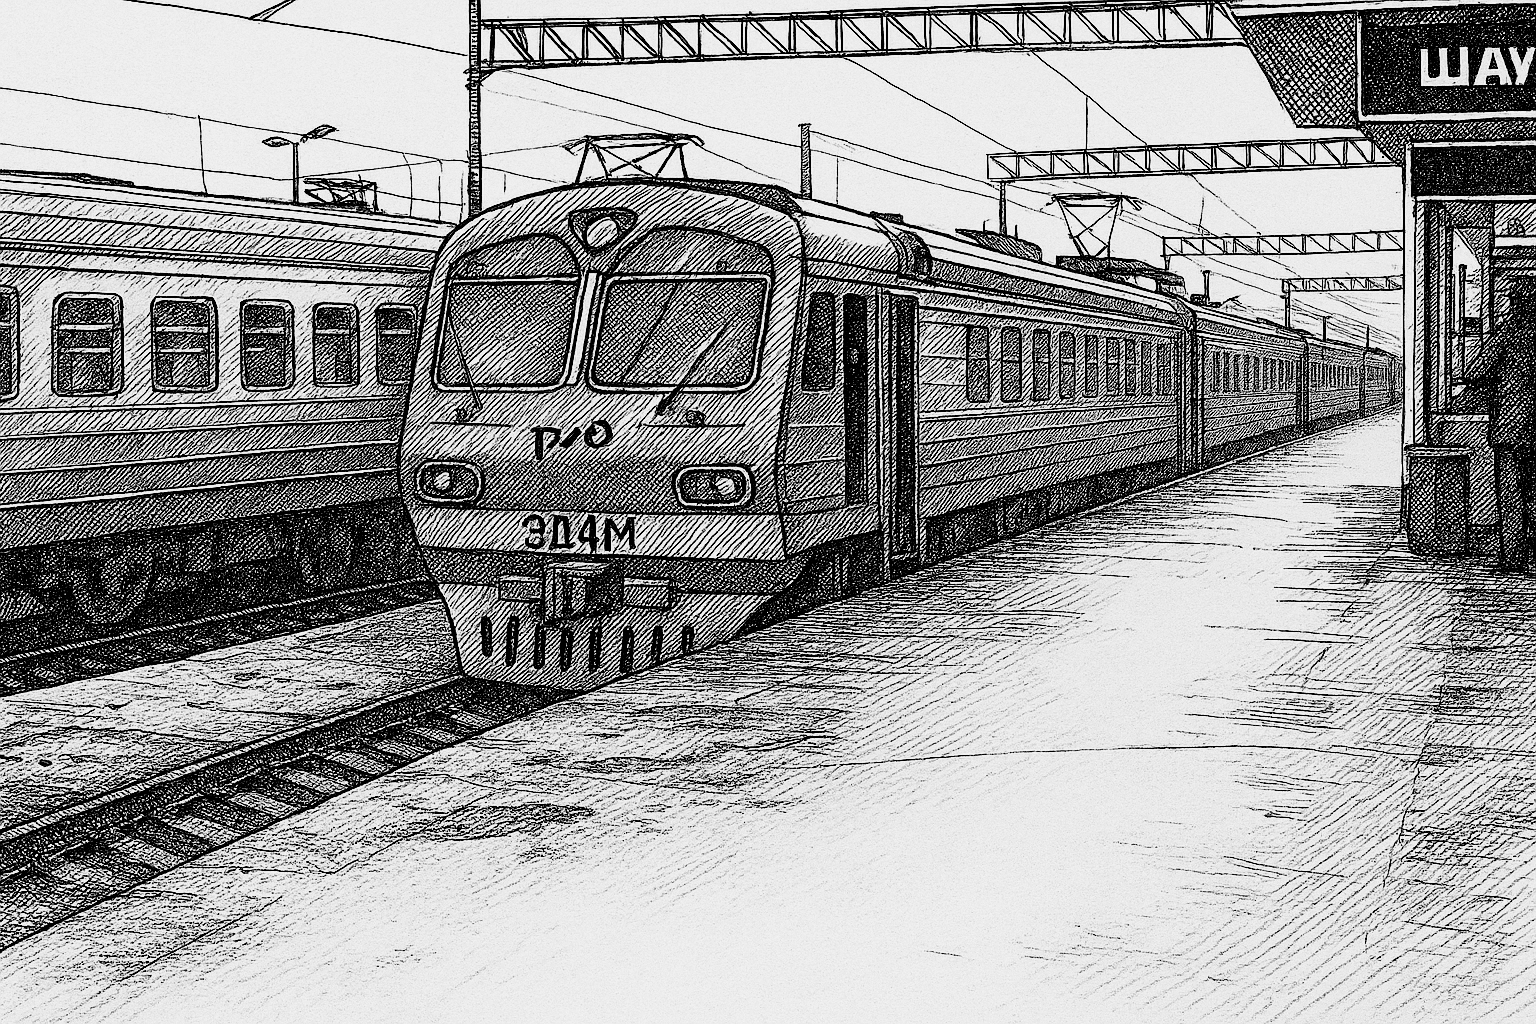
\includegraphics[width=1.0\textwidth]{1_new5}
			\caption{\small\textit{...в электричке c Курского вокзала...}}
			%	\end{wrapfigure} 
		\end{figure}
	}
	на~ушатанных стрелках. Хотелось тишины, покоя. Но~по~вагонам потянулись торговцы, большинство из них торговало тут годами. Один из них особенно нравился ему:	

	
	\diagdash Шариковые ручки по ценам брежневских времён! Самовывоз со склада в Антарктиде!\mdash вещал прокуренным голосом весельчак с трёхдневной седой щетиной.\mdash Я же, со своей стороны, гарантирую вам бесплатную доставку в любую точку$\ldots$\mdash мужик делал драматическую паузу, наслаждаясь производимым эффектом,\mdash $\ldots$вагона! Итак,~п\sdash жалста! Ручки по ценам брежневских времён!%$\ldots$
	
	Шурик прислонился к стеклу окна в вагоне и уныло посмотрел вслед уходящему мужичку с ручками. Как~тому безумно, должно быть, всё осточертело, думал он, как и~сотням тысяч людей вокруг$\ldots$ В вагон ввалилась следующая торговка и стала что\sdash то впаривать. Но разве можно было переплюнуть <<Антарктиду>>? 
		
%	\begin{wrapfigure}{r}{0.55\textwidth}
%		\centering
%		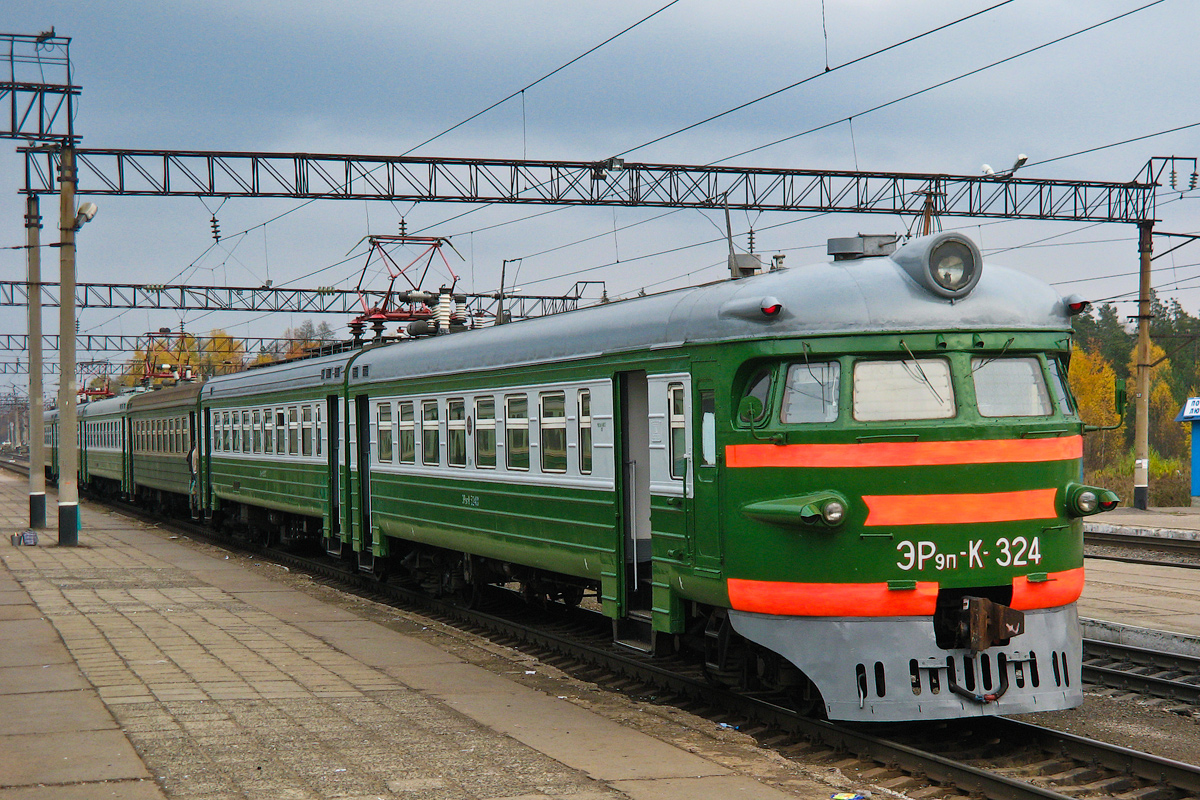
\includegraphics[width=0.55\textwidth]{1}
%	\end{wrapfigure}	
	Кое\sdash как Шурик дожил до вечера. И, вроде бы, ничего особенного не произошло\mdash рутинные будни текли как обычно\mdash но где\sdash то глубоко в груди уже зажёгся огонёк Нового Сплава. Его работа на <<почтовом ящике>>\footnote{Выражение советского периода, означающее предприятие оборонного значения; при переписке адрес обозначался <<почтовый ящик~№N>>.} была интересной, но никому не нужной, он знал это. Можно было попытаться сделать кандидатскую\mdash плюс три тысячи рублей к зарплате. <<Ага, и минус три тысячи из~премии, плавали, знаем!>>\mdash думалось ему с отвращением. Он~попытался было подёргаться по~смежным <<ящикам>>, но~сам процесс вызывал у него тоску\mdash эти проходные, эти оформления пропусков, эти коридоры, полные подковёрной борьбы, эти усталые, ни~во что особо не верящие люди$\ldots$ Одни <<ящики>> были ещё хуже, чем его, другие получше, но~сойтись с~людьми не получилось, характер у Шурика был не~сахар и он знал это. Знал и ничего не делал. Взбаломошное решение уволиться на вольные хлеба, попытка навсегда забыть это место, обернулось для него двухгодичным странноватым приключением по окончании которого он вновь привычно вернулся в русло своего многострадального <<ящика>>. Вернулся и снова принялся тянуть старую лямку под ухмылочки <<товарищей>>, но ему было уже всё равно. Болото <<ящика>> затягивало. Материал для кандидатской, при желании, можно было бы набрать, но мысли о никому не~нужной аспирантуре отталкивали от~этой затеи.%ля этого нужен был кто\sdash то, кому это будет нужно помимо Шурика\mdash руководитель. А Юрич, сам не будучи кандидатом, давно махнул на это рукой. 
	
	Ему вдруг так захотелось вздёрнуться, что он отвернулся к~стеклу, закрыв в бессильном забытьи глаза. За~окном проплыла очередная станция, скоро выходить.
	
	\diagdash День прошёл и х.. с ним.\mdash прошептал беззвучно он\mdash когда\sdash то услышанная фраза глубоко засела в его сознании. Получалась какая\sdash то концлагерная психология. Горизонт планирования\mdash до вечера. Дальше\mdash бессмысленно. Дальше\mdash страшно разочаровываться. Эти мысли вдруг ужаснули, обожгли. %Даже сейчас он как\sdash то с опаской прокручивал в голове всё насчёт сплава\mdash вдруг сорвётся? 
	
	Высыпавшись из электрички на~конечной, он побрёл домой, заглянув в магазин\mdash нужна была <<перезагрузка>>. В душ\'е желание просто сдохнуть боролось с желанием смотаться в поход или закрутить интрижку, чтобы хоть на немного вырваться из круга дом\nbdash электричка\nbdash работа\nbdash электричка\nbdash дом. Когда до~дому оставалось ещё минут пять ходу быстрым шагом, он остановился, стыдливо прикрыл тару и~<<перезагрузился>>$\ldots$
	
%	В душ\'е боролись примерно два чувства\mdash дикое желание сдохнуть и дикое желание пойти в~поход, чтобы не сдохнуть. Сопротивляться последнему день ото дня становилось просто невозможно. Такое вот единство и борьба противоположностей. 
	
%	\vspace{1.9cm}	
	$\ldots$Вечерело. Облачная, безветренная ночь проникала в~город.  Шурик вышел из квартиры в тапках на общий балкон, закутался в куртку, торопливо раскурил трубку и~набрал Замполиту своей команды\mdash Кире. Шурик уже и сам не помнил, почему он называл того Замполитом. Прилипло как\sdash то, вероятно, потому что Киря был опытным походником, байдарочником, и просто старым другом, на~которого можно было положиться в походе. Киря был его замом в нескольких предыдущих сплавах, в походах они были с ним <<на одной волне>>.

%	\newpage	
	Буквально со второго гудка Киря взял трубку:
	
	\diagdash Слушаю!
	
	\diagdash Кирь, такое дело, пошли в Карелию?\mdash немедленно, не~откладывая, выпалил Шурик, выпустив колечки из~трубочки.
	
	\diagdash Как два пальца. Когда?\mdash тот был бодр.
	
	\diagdash Ну как обычно, начало августа$\ldots$
	
	\diagdash До августа ещё дожить надо$\ldots$
	
	\diagdash Оптимист, ёпт! Короче\mdash все наши в теме, Юрич в~этот раз\mdash пас. Ты вписываешься?\mdash Шурику очень хотелось услышать простое и короткое согласие. Он~мысленно просто умолял Кирю согласиться сейчас же, без каких\sdash либо раздумий и~прочей чепухи\mdash тогда всё сразу станет ясно и понятно\mdash появится неоспоримая цель, сама суть, ради которой можно прожить до лета.
	
	\diagdash Шурик, я женюсь скоро.\mdash огорошил Киря.
	
	\diagdash Ё\sdash ё\sdash ё$\ldots$
	
	\diagdash Поэтому я и говорю\mdash до августа ещё дожить надо!
	
	Шурику вдруг стало невообразимо горько, что поход может снова, четвёртый год подряд, накрыться медным тазом, но в то же время радостно за Кирю\mdash таки женится\mdash возможно, удастся обрести кусочек семейного счастья\mdash островок спокойствия\mdash так~нужный, пожалуй, каждому. Грусть где\sdash то в недрах, катакомбах его души, нарастала как цунами. Вспомнились ему вдруг думы Маргариты: <<Только бы выбраться отсюда, а там уж я дойду до реки и утоплюсь>>\cite{МастерМаргарита}. Топиться в грязнющем соседнем пруду, где по осени наконец\sdash то потравили крыс, было как\sdash то не очень, и он посмотрел вниз с~балкона. <<10\sdash й этаж, пожалуй, хватит, чтоб уже наверняка>>,\mdash подумалось с грустью.
	
	Трубка потухла, снова раскуривать не захотелось, налетел какой\sdash то холодный ветер, настроение у него окончательно испортилось, и~Шурик, бессменный Адмирал Сплава, вышел с~балкона с~такой~же неопределённостью, как и заходил.
	
	Жена суетилась на кухне, запахи витали умопомрачительные. Он тихо снял куртку, вытряхнул потухшую трубку, хотел бесшумно проскользить в комнату. Паркет под его ногой скрипнул. 
	
	\diagdash Почисть картошки?\mdash бросила, услышав, с кухни жена.
	
	Шурик замер на предательской паркетине в коридоре.
	
	\diagdash Ты слышишь?\mdash уточнила жена. Интонации не~подразумевали промедления.
	
	\diagdash Да, сейчас$\ldots$
	
	Стоя у мойки и совершенно машинально счищая овощным ножом кожуру, Шурик мысленно унёсся в~Карелию$\ldots$ Это желанное место представлялось ему, почему\sdash то, чем\sdash то особенным. Исполинские сосны на~камнях, дождливая погода, рыба$\ldots$ Он даже прикрыл глаза, чистя картошку на ощупь. Внезапно он понял, что все эти предыдущие сплавы были лишь тренировкой перед Карелией, перед взятием порогов. А вокруг чтобы\mdash красивейшие берега с буйством растительности, скалы, видевшие ещё динозавров и неандертальцев, сосны с янтарной корой и~душистой хвоёй$\ldots$ От желания почувствовать это чуть не~закружилась голова. И чтобы людей вокруг\mdash ни души, только <<свои>>\mdash только своя бравая команда. Ух, парус с собой ещё взять по~озёрам походить$\ldots$ От одной только мысли о~парусе у~Шурика застучало в~висках.
	
	\diagdash Всё хорошо?\mdash спросила жена.
	
	\diagdash А? Да$\ldots$\mdash Шурик открыл глаза.
	
	\diagdash Кому звонил?
	
	\diagdash Кире.
	
	\diagdash Как он? 
	
	\diagdash Жениться надумал$\ldots$ 
	
	\diagdash А сам чего смурной? А, понятно! Вы опять намылились в поход, а тут такая подстава, да?\mdash ледяным взглядом скользнула жена, попав, словно снайперским выстрелом, точно в десятку.%.
	
	\diagdash В целом, да.\mdash не стал отпираться Шурик.
	
	\diagdash Всё образуется,\mdash пророчески сказала она и~вытащила из духовки ужин.\mdash Хрен вас кто удержит от~ваших пьянок на воде.
	
	Шурик хотел было устало прочитать ей лекцию о~технике безопасности распития в водном походе, но не стал.  На~душе у~него было так же холодно, как~в~Антарктиде.%$\ldots$ 
	
	\vspace{-0.2cm}
%	\noindent\textit{%
%		\hspace*{3.7cm}$\ldots$Без морозу, без огня,\\
%		\hspace*{3.7cm}Да сердце вызнобила,\\
%		\hspace*{3.7cm}Да рассыпала печаль\\
%		\hspace*{3.7cm}По моим ясным очам$\ldots$
%	}
%	
	\begin{center}
		\psvectorian[scale=0.4]{88} % Красивый вензелёк :)
	\end{center}
}